\documentclass{beamer}
\usetheme{Warsaw}

\fontfamily{pag}
\usepackage{libertine}
\usepackage{animate} %need the animate.sty file
\renewcommand*\familydefault{\sfdefault}

\setlength{\parskip}{1em}

\setbeamercolor{normal text}{fg=white,bg=black!90}
\setbeamercolor{structure}{fg=white}
\setbeamercolor{alerted text}{fg=red!85!black}
\setbeamercolor{item projected}{use=item,fg=black,bg=item.fg!35}
\setbeamercolor*{palette primary}{use=structure,fg=structure.fg}
\setbeamercolor*{palette secondary}{use=structure,fg=structure.fg!95!black}
\setbeamercolor*{palette tertiary}{use=structure,fg=structure.fg!90!black}
\setbeamercolor*{palette quaternary}{use=structure,fg=structure.fg!95!black,bg=black!80}
\setbeamercolor*{framesubtitle}{fg=white}
\setbeamercolor*{block title}{parent=structure,bg=black!60}
\setbeamercolor*{block body}{fg=black,bg=black!10}
\setbeamercolor*{block title alerted}{parent=alerted text,bg=black!15}
\setbeamercolor*{block title example}{parent=example text,bg=black!15}

%%%%%%%%%%%%%%%%%%%%%% 55
\setbeamertemplate{headline}{%
\leavevmode%
  \hbox{%
    \begin{beamercolorbox}[wd=\paperwidth,ht=4.8ex,dp=0.125ex]{primary}%
      \insertsectionnavigationhorizontal{\paperwidth}{}{\hskip0pt plus1filll}
    \end{beamercolorbox}%
  }
}

\usepackage{tikz}
\usetikzlibrary{shapes}
\setbeamertemplate{section in head/foot}{%
    \if\insertsectionheadnumber1
        \tikz\node[draw=gray,fill=gray,shape=signal,very thick,text=black]{\insertsectionhead\hskip.3cm};
    \else
        \tikz\node[draw=gray,fill=gray,shape=signal,signal from=west, signal to=east,very thick,text=black]     {\insertsectionhead\hskip.3cm};
  \fi
}

\setbeamertemplate{section in head/foot shaded}{%
    \if\insertsectionheadnumber1
        \tikz\node[draw=gray,fill=gray,shape=signal,very thick,text=black!30]{\insertsectionhead\hskip.3cm};
    \else
        \tikz\node[draw=gray,fill=gray,shape=signal,signal from=west, signal to=east,very thick,text=black!10]     {\insertsectionhead\hskip.3cm};
  \fi
}

%%%%%%%%%%5
\AtBeginSection[]{
  \begin{frame}
  \vfill
  \centering
  \begin{beamercolorbox}[sep=8pt,center,shadow=true,rounded=true]{title}
    \usebeamerfont{title}\insertsectionhead\par%
  \end{beamercolorbox}
  \vfill
  \end{frame}
}

\usepackage{grffile} %for underscores in file names
\usepackage{gensymb} % degree
\title{The Science of Brewing:}
\subtitle{How 4 simple ingredients become the best beverage in the world \newline \newline Part 3: \textbf{Water}}
\date{\footnotesize{\today}}
\author{Nick Waters}
\institute{Department of Microbiology\\
School of Natural Sciences\\
National University of Ireland, Galway}
\begin{document}
\maketitle


\section{Introduction}

\begin{frame}
\frametitle{Ingredients}
\begin{enumerate}
\item Barley
\item Hops
\item Water
\item Yeast
\end{enumerate}
\end{frame}

\begin{frame}
\begin{center}
    \hspace*{-10mm}\includegraphics[width=1.2\textwidth]{./brewing/overview.jpg}
\end{center}
\end{frame}

\begin{frame}
\frametitle{Disclaimer}
\begin{enumerate}
\item I am not an expert
\end{enumerate}
\end{frame}


\section{Water}

\begin{frame}\frametitle{Water}
\begin{center}
\includegraphics[width=.8\linewidth]{./brewing/water/Water_drop_001.jpg}
\end{center}
\end{frame}

\begin{frame}\frametitle{Water}
  \begin{itemize}
  \item Beer is $\approx$ 95\% water
    \item Water is flavorless; ions aren't
    \end{itemize}
\end{frame}

%%%%%%%%%%%%%%%%%%%%%

\section{Ions and their effect}

\begin{frame}\frametitle{Calcium}
    The most important ion in brewing!
    \begin{itemize}
    \item $ Ca^{+} + Ph[x] \rightarrow precipitate + H^{+} $
      \item low pH important for mash enzymes
      \end{itemize}
\end{frame}

\begin{frame}\frametitle{Magnesium}
  \begin{itemize}
  \item $ Mg \rightarrow happy yeast :) $
  \item Can give off-flavors in excess
  \end{itemize}
\end{frame}


\begin{frame}\frametitle{Sodium}
  \begin{itemize}
  \item accentuates flavor
    \item perceived sweetness
    \item off flavors when ossociating with sulfate ions
  \end{itemize}
\end{frame}

\begin{frame}\frametitle{Potassium}
  \begin{itemize}
  \item adds saltiness
    \item can inhibits mash enzymes
  \end{itemize}
\end{frame}

\begin{frame}\frametitle{Sulpher}
  \begin{itemize}
  \item Helps starch degradation
  \item Helps protein degradation (clarity)
    \item Negatively affects hopping
    \item Adds crispness to flavor, but off flavors in excess
  \end{itemize}
\end{frame}

\begin{frame}\frametitle{Phosphate}
  \begin{itemize}
  \item buffers pH when mashing and boiling
  \end{itemize}
\end{frame}

\begin{frame}\frametitle{Cholrides}
  \begin{itemize}
  \item NaCl MgCl both add body and sweetness
    \item useful for stouts, porters, belgium styles
  \end{itemize}
\end{frame}

\begin{frame}\frametitle{Carbonates}
  \begin{itemize}
  \item Raises pH
  \item Less fermentable and cloudy
    \item Can be used to correct for mash acidity
  \end{itemize}
\end{frame}

\begin{frame}\frametitle{Nitrates}
  \begin{itemize}
  \item can reduce fermentation
  \end{itemize}
\end{frame}

\begin{frame}\frametitle{Some examples}
  \begin{table}[]
    \begin{tabular}{l|llllll}
      &          $Ca^{+2}$      & $Mg^{+2}$ & $Na^{+}$ & $Cl^{-}$ & $SO_{4}^{-2}$ & Alkalinity \\
      \hline
      Dublin    & 16   & 2   & 8   & 14    & 12         & 32 ($CaCO_3$) \\
      Arlington & 23   & 6   & 23  & 38    & 25         & 51 ($HCO_3$)  \\
      Boston    & 5    & 1   & 34  & 23    & 7          & 41 ($HCO_3$)  \\
      Limerick  & 130  & 20  & 14  & 25    & 20         & 437 ($HCO_3$) \\
      \textbf{Galway}    & 240  & 11  & 15  & 32    & 22          & 334 ($HCO_3$)
    \end{tabular}
  \end{table}
\end{frame}

\section{What to do about it}
\begin{frame}\frametitle{Nitrates}
  \begin{itemize}
    \item Chalk – Calcium Carbonate ($CaCO_{3}$) -- boosts alkalinity for brewing dark beers

    \item Baking soda – Sodium Bicarbonate ($NaHCO_{3}$) -- boosts alkalinity and ammend sodium

    \item Gypsum – Calcium Sulfate ($CaSO_+4 * 2 H_{2}0$) enhances hop bittering

    \item Calcium Chloride ($CaCl_2 * 2 H_{2}0$) -- ammend  low chloride water

    \item Epsom salt – Magnesium Sulfate ($MgSO_4 * 7 H_{2}0$) -- enhances hop bittering; use Mg sparingly if at all.
  \end{itemize}
\end{frame}

\section{Today's Brew}

\begin{frame}\frametitle{Christmas Ale}
  \begin{columns}
    \begin{column}{.5\textwidth}
      Malt
      \begin{itemize}
      \item 5kg Irish Pale Malt (4-6)
      \item 1kg Crystal 30  (5)
      \item 500g Cara Special X  (20)
      \end{itemize}
      Yeast
      \begin{itemize}
      \item Safale T-58
      \item Wyyeast Belgium Ale
      \end{itemize}
      Protein rest 10 mins at 58\degree.
      Mash for 30 minutes at 63 \degree.
      Mash for 30 minutes at 65 \degree.
      Hot crash/sparge with 8 liters at 75\degree.
      Boil 70 minutes.  Target gravity: 1.072.
    \end{column}
    \begin{column}{.5\textwidth}
      Hop Additions:
    \begin{itemize}
    \item 60mins 50g Hallertauer and Sonnet
    \item 25g juniper berries
    \item flameout Hallertauer and Sonnet
    \item (\dots more juniper? )
    \end{itemize}
  \end{column}
\end{columns}
\end{frame}


%%%%%%%%%%%%%%%%%%%%%
%% \begin{frame}\frametitle{Hops}
%% \centering\includegraphics[width=\linewidth]{./brewing/hops/Cross-section-dark.pdf}
%% \end{frame}

%% \begin{frame}\frametitle{History of Hop Cultivation}
%%   \begin{itemize}
%%   \item Documented cultivation between 736--1079 in Hallertau, Germany
%%   \item Pepin the Short left hop gardens to Charlemagne in 768
%%   \item Hopped beer introduced to Britain in 1400
%%   \item Hops cultivated in England 1524
%%   \item Hops cultivated in America 1629
%%   \end{itemize}
%%   \centering\includegraphics[width=.5\linewidth]{./brewing/hops/bohemia}
%% \end{frame}

%% \begin{frame}\frametitle{Modern Cultivation}
%%   \begin{itemize}
%%   \item Dioecious: males not used for brewing
%%   \item Bines trained over strings on trestles
%%   \item Susceptible to mold and mildew
%%   \end{itemize}
%%   \centering  \includegraphics[width=.7\linewidth]{./brewing/hops/Hopfengarten.jpg}
%% \end{frame}



%% \section{Why hops?}

%% \begin{frame}\frametitle{Unhopped beer}
%%   \begin{columns}
%%     \begin{column}{0.6\textwidth}
%%     \begin{itemize}
%%     \item Yeast never 100\% effective; beer is sweet
%%     \item Gruit: bitter spice mixure: sweet gale, mugwort, yarrow, ground ivy, horehound, and Calluna heather, juniper berries, ginger, caraway seed, aniseed, nutmeg, cinnamon, etc.
%%     \item More expensive, more prone to spoilage
%%     \end{itemize}
%%   \end{column}
%%   \begin{column}{0.5\textwidth}
%%     \begin{center}
%%       \centering  \includegraphics[width=.7\linewidth]{./brewing/hops/Gruit-Mixture.jpg}
%%     \end{center}
%%   \end{column}
%%   \end{columns}
%%       \tiny{http://www.gruit.es/en/brewmaster-1a-part/}
%% \end{frame}

%% \begin{frame}\frametitle{Hopped beer}
%%   \begin{columns}
%%     \begin{column}{0.6\textwidth}
%%     \begin{itemize}
%%     \item Cheap
%%     \item Antibacterial properites
%%     \item Tasty!
%%     \end{itemize}
%%   \end{column}
%%   \begin{column}{0.5\textwidth}
%%     \begin{center}
%%       \centering  \includegraphics[width=\linewidth]{./brewing/hops/Hopfendolde-mit-hopfengarten.jpg}
%%     \end{center}
%%   \end{column}
%%   \end{columns}
%% \end{frame}

%% \section{What's in Hops?}


%% \begin{frame}\frametitle{Hops are:}
%%   % \begin{itemize}
%%   % \item alpha acids
%%   % \item beta acids
%%   % \item oils
%%   % \item flavenoids
%%   % \item other stuff
%%   % \end{itemize}
%% \begin{table}[]
%% \centering
%% \label{components}
%% \begin{tabular}{lr}
%%   \textbf{Components} & \textbf{(\%w/w)} \\
%%   Cellulose + lignin & 40.0 \textemdash 50.0 \\
%%   Protein & 15.0 \\
%%   {\color{green}$\alpha$ acids} & 2.0 \textemdash 17.0  \\
%%   {\color{green}$\beta$ acids} & 2.0 \textemdash 10.0 \\
%%   Minerals & 8.0 \\
%%   Polyphenols and tannins & 3.0 \textemdash 6.0 \\
%%   Lipids and fatty acids & 1.0 \textemdash 5.0 \\
%%   {\color{green}Hop oil} & 0.5 \textemdash 3.0 \\
%%   Monosaccharides & 2.0 \\
%%   Pectin & 2.0\\
%% \end{tabular}
%% \end{table}
%% \tiny{European Brewery Convention Hops and Hop Products, Manual of Good Practice; Getranke - Fachverlag Hans Carl: Nurnberg, Germany, 1997. Water not shown}
%% \end{frame}

%% % \begin{frame}\frametitle{$\alpha$ acids (Humulones)}
%% %   \centering
%% %   \animategraphics[autoplay,loop,controls,poster=last,height=3.9cm]{100}{brewing/hops/animations/humulone_}{0}{179}

%% % \end{frame}


%% \begin{frame}\frametitle{$\alpha$ acids (Humulones)}
%%   \includegraphics[width=.85\textwidth]{./brewing/hops/isomerization.jpg}
%%   \begin{itemize}
%%   \item Bitter (IBU measuring)
%%   \item Antimicrobial
%%   \item ``skunking'': sun + isohumulones $\rightarrow$ free radicals $\rightarrow$ thiols
%%     \item Good bitterness
%%   \end{itemize}
%% \end{frame}


%% \begin{frame}\frametitle{$\beta$ acids (Lupulones)}
%%   \includegraphics[width=.5\textwidth]{./brewing/hops/Lupulone-dark.pdf}
%%   \begin{itemize}
%%     \item Bad bitterness
%%   \end{itemize}
%% \end{frame}

%% \begin{frame}\frametitle{Essential Oils}
%%   \begin{columns}
%%     \begin{column}{0.6\textwidth}
%%       Myrcene
%%       \begin{itemize}
%%       \item Thyme, cannabis, lemmongrass, bay leaf, mango, lavender
%%       \item Aromatic, but unstable; prone to Diels-Alder reactions
%%       \end{itemize}
%%       Humulene
%%       \begin{itemize}
%%       \item Ginger, cannabis, orange, pine, sage, tobacco
%%       \item Lends aroma;  especially high percentage in Noble hops
%%       \end{itemize}
%%       Caryophyllene
%%       \begin{itemize}
%%       \item Black pepper, cannabis, caraway, cloves, oregano, rosemary
%%       \end{itemize}
%%     \end{column}

%%     \begin{column}{0.4\textwidth}
%%       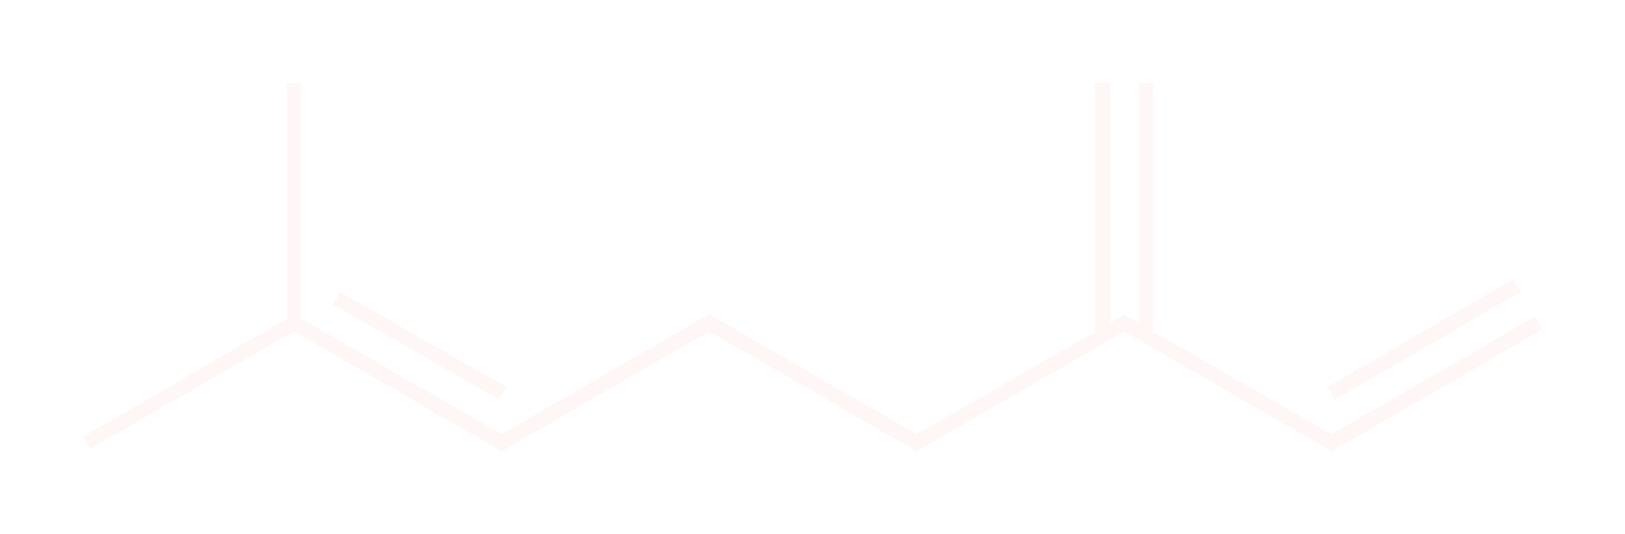
\includegraphics[width=.8 \textwidth]{./brewing/hops/Myrcene-dark.pdf}
%%       \includegraphics[width=0.5\textwidth]{./brewing/hops/Humulene-dark.pdf}
%%       \includegraphics[width=.6\textwidth]{./brewing/hops/Beta-Caryophyllen-dark.pdf}
%%     \end{column}
%%   \end{columns}
%% \end{frame}

%% \begin{frame}\frametitle{Flavenoids}
%%   \begin{columns}
%%     \begin{column}{.6\textwidth}
%%       Xanthohumol
%%       \begin{itemize}
%%       \item Ends up about about 2 μg/L – 1.2 mg/L
%%       \item most abundant flavenoid in hops
%%       \item Contributes bitterness and flavor
%%       \end{itemize}
%%       8-Prenylnaringenin phytoestrogen

%%     \end{column}
%%     \begin{column}{.4\textwidth}
%%       
\includegraphics[width=.8\textwidth]{./brewing/hops/Xanthohumol.pdf}
%%       \vspace{5mm}
%%       \includegraphics[width=.8\textwidth]{./brewing/hops/Sophoraflavanone_B-dark.pdf}
%%     \end{column}
%%   \end{columns}
%% \end{frame}



%% \section{The Pursuit of Hoppiness}
%% \begin{frame}\frametitle{Internation Bittering Units}
%%   IBUs: isomerized $\alpha$ acid content
%%   \begin{table}[]
%%     \centering
%%     \label{my-label}
%%     \begin{tabular}{lr}
%%       \textbf{Beer style} & \textbf{IBUs} \\
%%       Lambic              & 0-10          \\
%%       Wheat beer          & 8-18          \\
%%       American lager      & 8-26          \\
%%       Pilsner             & 24-44         \\
%%       Porter              & 18-50         \\
%%       Pale ale            & 30-50         \\
%%       Stout               & 30-90         \\
%%       Barleywine          & 34-120        \\
%%       India pale ale      & 40-120
%%     \end{tabular}
%%   \end{table}
%% \end{frame}

%% \begin{frame}\frametitle{How to hop}
%% \begin{table}[]
%% \centering
%% \begin{tabular}{rll}
%%   \textbf{Time} & \textbf{Type} & \textbf{Purpose}   \\
%%   \hline
%% 30-90 & bitterness & conversion of $\alpha$ acids  \\
%% 10-30 & flavour & extraction of oils and other volatile compounds  \\
%% 0-10 & aroma & extraction of delicate, volatile compounds \\
%% ... & dry & slow extraction of oils and other compounds \\
%% \end{tabular}
%% \end{table}
%% \end{frame}

%% \section{Hop Varieties}
%% \begin{frame}\frametitle{Notable Hops}
%%   Noble Hops
%%   \begin{itemize}\vspace{-4mm}
%%   \item The OG cultivars: Hallertau, Tettnanger, Spalt, and Saaz
%%   \item  Pilsen Urquell,  Stella Artois
%%   \end{itemize}
%%   British Noble Hops
%%   \begin{itemize}\vspace{-4mm}
%%   \item Fuggle, East Kent Goldings and Goldings
%%   \item Guineess, Smithwicks
%%   \end{itemize}
%%   New World Hops
%%   \begin{itemize}\vspace{-4mm}
%%   \item Cascade, Chinook, Nugget, Citra, Simcoe, Willamette
%%   \item IPAs
%%   \end{itemize}
%%   Pacific Hops
%%   \begin{itemize}\vspace{-4mm}
%%   \item Nelson Sauvin, Pacifica, Pacific Gem, Super Alpha
%%   \end{itemize}
%% \end{frame}

%% % hop plot #1
%% % hop plot #1
%% % brewing plan
%% \section{Sources}
%% \begin{frame}
%%   \begin{itemize}
%%   \item \url{http://onlinelibrary.wiley.com/doi/10.1002/jib.160/pdf}
%%   \item \url{http://www.uvm.edu/extension/cropsoil/wp-content/uploads/2014HopsConference_Shellhammer_brewersperspective.pdf}
%%   \item wikipedia (lots of wikipedia)
%%   \end{itemize}
%% \end{frame}



\end{document}
